% ============================================================
%  PPAM 2026 - Springer LNCS template
%  Requires: llncs.cls
% ============================================================
\documentclass{llncs}

% ---- Core packages ----------------------------------------
\usepackage[hyphens]{url}
\usepackage{graphicx}
\usepackage{booktabs}
\usepackage{amsmath}
\usepackage{amssymb}
\usepackage{multirow}
\usepackage{xcolor}
\usepackage{siunitx}
\usepackage{microtype}
\usepackage{etoolbox}
\usepackage{float}
\usepackage{placeins}
\usepackage[caption=false]{subfig}
\usepackage{needspace}

% NOTE: \l (Polish ł) is illegal inside \hyphenation{}, so Przemysław
%       is protected with \mbox{} at its two occurrences in the text.
\hyphenation{%
  Dz-wi-nel            % Polish name: Dz/wi/nel
  back-prop-a-ga-tion  % prevents ugly back-\npropagation split
  hy-per-pa-ra-me-ter  % prevents hy-\nperparameter at line end
  reg-u-lar-i-sa-tion  % UK English form used throughout
  re-pro-du-ci-bil-i-ty
}

\urlstyle{rm}

% Float placement - allow floats to occupy more of the page
\renewcommand{\topfraction}{0.9}
\renewcommand{\bottomfraction}{0.8}
\renewcommand{\textfraction}{0.05}
\renewcommand{\floatpagefraction}{0.8}

% Widow/club/hyphen penalties
\clubpenalty=9000
\widowpenalty=9000
\hyphenpenalty=500
\emergencystretch=1em

\setlength{\textfloatsep}{12pt plus 2pt minus 2pt}

% siunitx custom unit
\DeclareSIUnit\mebibyte{MiB}

\sisetup{
  table-sign-mantissa,
  table-align-comparator=false,
  detect-weight=true,
  detect-family=true
}

% Algorithm name macros
\newcommand{\FF}{\texttt{FF}}
\newcommand{\MF}{\texttt{MF}}
\newcommand{\BP}{\texttt{BP}}
\newcommand{\CaFo}{\texttt{CaFo}}
\newcommand{\CaFoRand}{\texttt{CaFo-Rand}}
\newcommand{\CaFoDFA}{\texttt{CaFo-DFA}}

\setcounter{secnumdepth}{2}

% ============================================================
%  Title, authors, institute
% ============================================================
\title{Energy-Efficient Deep Learning Without Backpropagation:\\
A~Rigorous Hardware-Validated Benchmarking Study of Forward-Only
Algorithms}

\author{Przemys{\l}aw Spyra\inst{1}\orcidID{0009-0009-3001-2604} \and
Witold Dzwinel\inst{1}\orcidID{0000-0001-8321-5928}}
\titlerunning{Energy-Efficient Deep Learning Without Backpropagation}
\authorrunning{P. Spyra and W. Dzwinel}

\institute{AGH University of Krakow, Faculty of Computer Science\\
\email{przspyra@agh.edu.pl, dzwinel@agh.edu.pl}}

% ============================================================
\begin{document}
\maketitle
% ============================================================

\begin{abstract}
Backpropagation (\BP{}) remains the dominant algorithm for training deep
neural networks, yet its high memory and energy costs motivate the
search for practical alternatives. We present a rigorous,
hardware-validated benchmarking study of three forward-only,
BP-free training algorithms, namely Forward-Forward (\FF{}), Cascaded Forward
(\CaFo{}), and Mono-Forward (\MF{}), evaluated against a fairly tuned \BP{}
baseline on MLP and 3-block CNN architectures across four standard
vision benchmarks (MNIST, Fashion-MNIST, CIFAR-10, CIFAR-100). Using a
principled comparison framework with identical architectures, universal
hyperparameter optimisation via Optuna, and direct hardware-level
efficiency measurement via the NVIDIA Management Library (NVML), we
find that \MF{} consistently matches
or surpasses \BP{} in classification accuracy on its native MLP
architectures, achieving up to 41\% lower energy consumption
and up to 34\% faster training on these configurations. We
further conduct an empirical re-evaluation of memory efficiency,
demonstrating that practical overhead can offset theoretical savings
from eliminating the backward pass. These findings are specific to MLP
architectures on standard benchmarks; performance on CNNs, transformers,
or larger-scale settings remains an open question. Our primary
contribution is the benchmarking framework itself and, to our knowledge,
the first hardware-validated comparison of \MF{} against a fairly tuned \BP{}
baseline under controlled conditions.
\end{abstract}

\begin{keywords}
backpropagation-free learning \and forward-only algorithms \and energy
efficiency \and hardware benchmarking \and deep neural networks
\end{keywords}

% ============================================================
\section{Introduction}
% ============================================================

Deep neural networks (DNNs) have achieved transformative success across
AI~\cite{krizhevsky2012imagenet,he2016deep,devlin2019bert}, yet this
progress rests on an escalating and unsustainable energy budget. As
models scale, their operational requirements are projected to consume
between 3\% and 4\% of global electricity by
2030~\cite{wef2025paradox}.

Training costs can be substantial: \cite{strubell2019energy} estimated
that training a single large Transformer with neural architecture search
produces roughly \SI{284}{\tonne} of CO$_2$e, comparable
to the lifetime emissions of five average American cars, while
\cite{patterson2021carbon} reported that training GPT-3 produced
approximately \SI{552}{\tonne} of CO$_2$e.

Among the algorithmic contributors to training energy costs,
backpropagation (\BP{})~\cite{rumelhart1986learning} plays a central
role. \BP{}'s dependence on a full backward pass necessitates storing all
intermediate activations, leading to memory costs proportional to
network depth. Its sequential, layer-locked nature imposes a
``backward locking'' bottleneck that constrains parallelisation and
prolongs training~\cite{jaderberg2017decoupled}.

These limitations motivate a search for alternatives drawing partial
inspiration from biological neural systems: local learning rules, the
absence of a global backward error signal, and layer-by-layer credit
assignment. None of the algorithms studied here claim full biological
plausibility~\cite{lillicrap2020backpropagation}; the \FF{}
algorithm~\cite{hinton2022forward} was explicitly motivated by these
considerations, and \MF{}'s local projection mechanism shares structural
similarities with local learning rules. We note these connections as
motivating context rather than as validated claims.

This paper investigates three forward-only algorithms that partially
instantiate such local principles:
\begin{itemize}
  \item \textbf{Forward-Forward (\FF{})}~\cite{hinton2022forward}, a
        foundational proof of concept demonstrating the viability of
        local, forward-only learning via a contrastive ``goodness''
        objective.
  \item \textbf{Cascaded Forward (\CaFo{})}~\cite{zhao2023cafo}, a
        structured evolution employing block-wise local classifiers to
        provide more direct supervisory signals.
  \item \textbf{Mono-Forward (\MF{})}~\cite{gong2025mono}, a refinement
        using per-layer projection matrices and local cross-entropy
        losses to improve accuracy and training efficiency.
\end{itemize}

While the potential of these algorithms is recognised in the literature,
a comprehensive and fair evaluation based on direct hardware-level
energy metrics has been insufficiently explored. Existing comparisons
often overlook architectural differences or inconsistent tuning
practices, which can confound algorithmic
comparisons~\cite{desislavov2024energy}. This paper addresses this gap
by conducting a systematic, hardware-validated benchmarking comparison
of \FF{}, \CaFo{}, and \MF{} against fairly tuned \BP{} baselines on their
respective native architectures. This benchmarking and hardware
characterisation contribution is directly relevant to the PPAM focus on
parallel and applied computing.

\paragraph{Contributions.}
The main contributions of this work are:
\begin{itemize}
  \item \textbf{A Rigorous Comparative Benchmarking Framework:} We
        establish a transparent, reproducible framework mandating
        identical native architectures, universal hyperparameter tuning
        applied equally to all methods, and direct hardware-level
        efficiency measurement via NVML\@. This framework is itself a
        transferable contribution for future BP-free evaluations.
  \item \textbf{Hardware-Validated Benchmarking of \MF{}:} To our
        knowledge, the first hardware-validated comparison of the
        Mono-Forward algorithm against a fairly tuned \BP{} baseline under
        controlled conditions, finding that \MF{} matches or surpasses \BP{}
        in accuracy on MLP architectures while achieving up to 41\%
        lower energy consumption on certain configurations.
  \item \textbf{Empirical Re-evaluation of Memory Efficiency:} We
        demonstrate that practical implementation overhead can offset
        the theoretical memory savings from eliminating the backward
        pass, correcting a common assumption in the BP-free literature.
\end{itemize}

% ============================================================
\section{BP-Free Training Algorithms}
\label{sec:algorithms}
% ============================================================

The high memory cost, sequential backward locking, and lack of
biological plausibility of backpropagation have motivated a search for
alternative training
paradigms~\cite{lillicrap2020backpropagation,jaderberg2017decoupled}.
This section describes the three algorithms evaluated in this work.

\paragraph{Forward-Forward (FF).}
Proposed by Geoffrey Hinton, the \FF{} algorithm~\cite{hinton2022forward}
replaces the forward and backward passes of \BP{} with two forward passes:
one using ``positive'' (real) data and another using ``negative''
(contrastive) data. Each layer learns locally to maximise a
layer-specific ``goodness'' metric on positive data while minimising it
on negative data, enabling purely local credit assignment. By
eliminating the global backward pass, \FF{} demonstrated that effective
representation learning is possible with local objectives. Its
contrastive design partially instantiates the biological principle of
Hebbian-like, local synaptic
modification~\cite{journe2023hebbian}. However, generating meaningful
negative samples and the indirect goodness signal were identified as
practical limitations, often leading to slow convergence and inefficient
hardware utilisation~\cite{hinton2022forward,zhao2023cafo}.

\paragraph{Cascaded Forward (CaFo).}
The \CaFo{} algorithm~\cite{zhao2023cafo} introduces a block-wise
framework of cascaded neural blocks, each followed by a local auxiliary
classifier. This provides direct cross-entropy supervision at multiple
network depths, eliminating the need for negative samples. Neural
blocks can be randomly initialised and fixed (\CaFoRand{}) or
pretrained with Direct Feedback Alignment (\CaFoDFA{}). While
\CaFo{} improves upon \FF{}'s indirect supervision, \CaFoRand{}
suffers from poor feature quality on complex tasks, while
\CaFoDFA{} improves accuracy at a significant computational cost
for block pretraining.

\paragraph{Mono-Forward (MF).}
\MF{}~\cite{gong2025mono} simplifies and enhances the local learning
mechanism by equipping each hidden layer with a dedicated, learnable
projection matrix. This matrix maps the layer's activations directly to
class-specific goodness scores, upon which a standard cross-entropy loss
is computed locally. Both the layer's primary weights and its projection
matrix are updated using only this local loss signal, enabling a single,
clean forward pass during training. This mechanism is structurally
similar to the local losses framework of \cite{ren2023scaling}, which
demonstrated that forward-gradient methods augmented with local
auxiliary losses scale favourably. \MF{} reportedly achieves accuracy
matching or surpassing \BP{} on MLP architectures, which motivated the
rigorous validation in this work.

% ============================================================
\section{Related Work}
\label{sec:related_work}
% ============================================================

\paragraph{Forward-Only and Local-Loss Methods.}
The foundational \FF{} algorithm~\cite{hinton2022forward} has inspired
multiple improvements. \cite{papachristodoulou2024convolutional}
introduced convolutional channel-wise competitive learning for \FF{},
extending it to CNN architectures with improved feature quality, a
limitation our experiments confirm for the base \FF{} method.
\cite{lorberbom2024layer} proposed collaborative layer objectives that
allow layers to share information during \FF{} training, reducing the
isolation inherent in purely local objectives. Both works report
improved accuracy over baseline \FF{} on standard benchmarks but do not
provide hardware-level efficiency comparisons of the kind conducted
here.

\cite{ren2023scaling} demonstrated that forward gradient methods
augmented with local auxiliary losses scale well, providing theoretical
and empirical grounding for \MF{}'s local projection approach; their work
focuses on scalability to larger models, whereas we focus on
hardware-level efficiency under fair experimental conditions.
\cite{journe2023hebbian} proposed Hebbian learning as a biologically
motivated alternative to \BP{}, while \cite{malladi2023fine} demonstrated
forward-only fine-tuning of large language models via memory-efficient
zeroth-order optimisation (\texttt{MeZO}) — a different regime (large
pretrained models, gradient estimation) than ours (training from
scratch, local deterministic losses), but one that contextualises the
broader hardware implications of BP-free training.

\paragraph{Predictive Coding.}
Predictive coding offers another biologically motivated alternative to
\BP{}\@. \cite{salvatori2022associative} demonstrated that predictive
coding networks can serve as associative memory solvers, and
\cite{salvatori2022brain} contextualise where local learning methods
fit within the broader landscape of brain-inspired learning.
\cite{pinchetti2022predictive} extended predictive coding beyond
Gaussian assumptions, while \cite{salvatori2024stable} introduced a
stable, fully automatic variant achieving competitive performance across
diverse tasks. Unlike the methods we evaluate, predictive coding
networks maintain explicit generative models of their inputs, incurring
different computational trade-offs.

\needspace{4\baselineskip}
\paragraph{Local Loss Optimisation Theory.}
\cite{ishikawa2025local} analysed local loss optimisation in the
infinite-width limit, providing theoretical grounding for why greedy
layer-wise training can generalise well. Their analysis supports the
hypothesis (Section~\ref{sec:discussion_why_mf}) that \MF{}'s layer-wise
training may act as a form of regularisation, though we treat this as a
hypothesis requiring further empirical investigation rather than a
confirmed result.

\paragraph{Hardware and Energy Considerations.}
BP-optimised hardware accelerators, including GPUs and
TPUs~\cite{jouppi2017datacenter}, are designed around the
forward--backward pass structure of \BP{}\@. \cite{strubell2019energy}
and \cite{patterson2021carbon} provide empirical grounding for the
energy costs of current BP-based training, situating our efficiency
comparisons within a broader sustainability context.

\paragraph{Positioning This Work.}
The present study complements the above by providing what is, to our
knowledge, the first hardware-validated benchmarking comparison of \FF{},
\CaFo{}, and \MF{} under a strictly controlled fairness framework: identical
architectures, universal hyperparameter tuning, and direct NVML energy
measurement. We do not introduce new algorithms; our contribution is
evaluative.

% ============================================================
\section{Framework for Fair and Rigorous Comparison}
\label{sec:framework}
% ============================================================

As a key contribution, we propose a rigorous benchmarking framework
designed to isolate the impact of the training algorithm from
confounding variables. Throughout, a \emph{hardware-validated
comparison} is one in which every efficiency claim is backed by a
physical quantity read from the GPU itself while the workload runs —
energy, elapsed time and memory occupancy — rather than by an
analytical proxy such as a FLOP or parameter count.

\paragraph{Fairness Protocols.}
A strict set of protocols was adhered to for all experiments:
\begin{enumerate}
  \item \textbf{Native Architecture Replication:} Each algorithm was
        implemented on its native architecture as described in its
        source publication. \FF{} and \MF{} were evaluated on their designated
        MLP structures; \CaFo{} on its defined 3-block CNN\@. CIFAR inputs
        are flattened to 1-D vectors for MLP experiments, following the
        original \MF{} protocol.
  \item \textbf{Identical Architectures for \BP{} Baselines:} For each
        experiment, a \BP{} baseline was constructed using an \emph{identical}
        network architecture, omitting only algorithm-specific components
        (e.g., goodness heads, projection matrices).
  \item \textbf{Systematic and Universal Hyperparameter Tuning:}
        Optuna~\cite{akiba2019optuna} was applied to \emph{all}
        algorithms, namely \FF{}, \CaFo{}, \MF{}, and their \BP{} baselines, for every
        configuration, maximising validation set accuracy. Full Optuna
        search spaces are in the supplementary material.
  \item \textbf{Consistent Early Stopping:} Training was governed by a
        consistent early stopping protocol based on validation
        performance~\cite{prechelt1998early}.
  \item \textbf{Fixed Random Seeds:} All sources of randomness were
        fixed. Three independent runs used seeds 42, 123, and 7. Full
        seeding and augmentation details are in
        the supplementary material.
\end{enumerate}

\paragraph{Note on Baseline Completeness.}
The absence of a \BP{} baseline augmented with per-layer auxiliary
classification heads (\texttt{BP-DS}) is a key limitation of the
current design; the full discussion and implications are given in
%
% FIX #1: Corrected from "Limitation~7" to "Limitation~6".
% The missing BP-DS baseline is the sixth enumerated item in §6.4;
% Limitation~7 is the inconsistent Fashion-MNIST MF result.
%
Limitation~6 (Section~\ref{sec:limitations}).

\paragraph{Architecture and Optimiser Configuration.}
All layer weights and projection matrices were initialised with Kaiming
uniform initialisation. \BP{} baselines were trained with AdamW, while
\CaFo{} predictors and \MF{} layers used Adam on a local cross-entropy
loss. Each \CaFo{} block comprises a $3{\times}3$ convolution, ReLU,
$2{\times}2$ max-pooling and batch normalisation, with 32, 128 and 512
output channels respectively; the three block-wise predictors are
aggregated by summation to form the final prediction. \FF{} used a fixed
goodness threshold $\theta=2.0$ with peer normalisation (factor 0.03,
momentum 0.9). \MF{} used a weight decay fixed at 0.0, leaving the
learning rate and the number of epochs per layer as the tuned
quantities. Optuna searched the remaining learning rates and weight
decays for every algorithm and every \BP{} baseline; the search spaces
and selected values are in the supplementary material.

\paragraph{Experimental Setup.}
Experiments were conducted on MNIST~\cite{lecun1998gradient},
Fashion-MNIST~\cite{xiao2017fashion}, CIFAR-10, and
CIFAR-100~\cite{krizhevsky2009learning}. All experiments ran on
NVIDIA A100-SXM4-40GB GPUs (Athena cluster, ACK Cyfronet AGH), hosted on
AMD EPYC 7742 nodes running Rocky Linux~9.8 with NVIDIA driver
595.71.05, Python~3.10.4 and PyTorch~v2.4.0. The system CUDA toolkit
version was 12.4.0; the PyTorch wheel (\texttt{torch==2.4.0+cu121})
bundles a CUDA~12.1 runtime. The driver version is stated because it
governs NVML power-reading semantics; NVML energy readings are obtained
via the system driver and are not affected by the runtime version
difference.
Full environment details are in the supplementary material.

For CIFAR-10 and CIFAR-100, standard training augmentation was applied
consistently to all algorithms \emph{and} their \BP{} baselines: random
horizontal flips ($p{=}0.5$) and random $32{\times}32$ crops with
4-pixel padding. CIFAR inputs for MLP architectures were flattened to
1-D vectors following the \MF{} protocol~\cite{gong2025mono}, with
augmentation applied before flattening. No augmentation was applied to
MNIST or Fashion-MNIST (see the supplementary material for full details).

\paragraph{Evaluation Metrics.}
Energy and memory were captured with NVML, the vendor-supplied library
that exposes the GPU's own power, clock and memory telemetry to a host
process; it was chosen because it reports what the device actually drew
and occupied, so no modelling assumption about the workload enters the
efficiency figures. The full metric suite is:
\begin{itemize}
  \item \textbf{Performance:} Test-set classification accuracy
        (mean~$\pm$~std across three independent runs).
  \item \textbf{Efficiency (Direct Measurement):} Training time
        (\si{\second}), energy consumption (\si{\watt\hour}, via NVML),
        and peak GPU memory (\si{\mebibyte}, via NVML). Exact NVML API
        usage is in the supplementary material.
  \item \textbf{Estimated CO$_2$e and GFLOPs
        (Repository Only):} Available at the public
        repository;
        omitted from the main paper due to methodological dependencies
        that would require separate treatment.
\end{itemize}

% ============================================================
\section{Experiments and Results}
\label{sec:experiments}
% ============================================================

The experiments reveal a progression among BP-free algorithms with
distinct accuracy--efficiency trade-offs, culminating in \MF{}'s favourable
profile on MLP architectures. Results are reported as
mean~$\pm$~standard deviation across three independent runs
(seeds~42,~123,~7).

% ---- 5.1 ---------------------------------------------------
\needspace{3\baselineskip}
\subsection{\FF{}: A Conceptually Sound but Computationally Costly
Starting Point}

{\looseness=-1
The experiments confirmed that \FF{} achieves competitive accuracy on its
native MLP architectures, validating its core premise. However, this
comes at a prohibitive efficiency cost
(Table~\ref{tab:ff_bp_mlp_summary}), with slow and volatile convergence
causing up to a~13$\times$ longer training time (Fashion-MNIST
4$\times$2000; see supplementary material) and nearly
10$\times$ greater energy use on the same configuration
compared to the \BP{} baseline.
The accuracy advantage over \BP{} was modest ($\leq$0.75~pp) and the
efficiency penalty was severe, raising the question of whether the
accuracy margin justifies the cost.
\par}

\begin{table}[tb]
  \centering
  \caption{Performance and efficiency: \FF{} vs.\ \BP{} on the
    Fashion-MNIST 4$\times$2000 MLP (mean~$\pm$~std, 3~runs;
    seeds 42, 123, 7). Better result in each column is shown in
    \textbf{bold}. Time and Energy cover full training to early
    stopping. Memory is peak GPU allocation reported by NVML\@.}
  \label{tab:ff_bp_mlp_summary}
  \setlength{\tabcolsep}{4pt}%
  \small
  \begin{tabular}{l
      S[table-format=2.2] @{\,$\pm$\,} S[table-format=1.2]
      S[table-format=3.2] @{\,$\pm$\,} S[table-format=2.1]
      S[table-format=2.2] @{\,$\pm$\,} S[table-format=1.2]
      S[table-format=4.0] @{\,$\pm$\,} S[table-format=1.0]}
    \toprule
    {Algorithm} &
      \multicolumn{2}{c}{Accuracy (\%)} &
      \multicolumn{2}{c}{Time (\si{\second})} &
      \multicolumn{2}{c}{Energy (\si{\watt\hour})} &
      \multicolumn{2}{c}{\shortstack[c]{Peak Mem \\ (\si{\mebibyte})}} \\
    \midrule
    \FF{}-AdamW    & \bfseries 89.63 & \bfseries 0.14 & 574.60 & 22.4 & 14.28 & 0.57 & 1190 & 8 \\
    \BP{} Baseline & 88.88 & 0.08 & \bfseries 43.09 & \bfseries 1.2 & \bfseries 1.48 & \bfseries 0.05 & \bfseries 1168 & \bfseries 4 \\
    \bottomrule
  \end{tabular}
\end{table}

The cost is not a matter of power draw
(Figure~\ref{fig:ff_convergence_dynamics}): \FF{} and \BP{} sit at comparable
wattage, and \FF{}'s energy bill is run up almost entirely by how long it takes
to reach its stopping criterion. The hardware-level reading of the
Fashion-MNIST configuration in Figure~\ref{fig:ff_resource_utilization} rules
out the obvious alternative explanations. Both algorithms hold the SM clock
near its ceiling throughout, so the penalty is not throttling. And on both
instruments---NVML device-wide and the \texttt{torch} allocator---\FF{}
consumed slightly \emph{more} peak memory than \BP{}, refuting a key presumed
advantage.

\begin{figure}[tb]
  \centering
  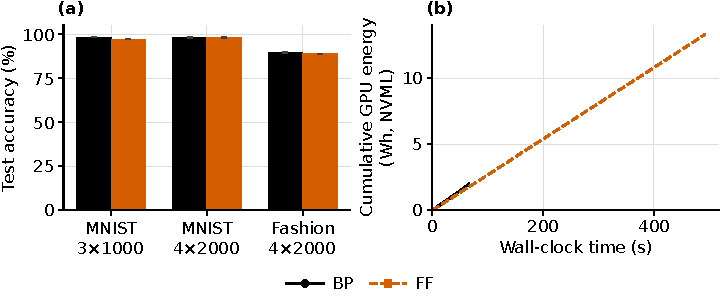
\includegraphics{plots/generated/fig_ff_cost.pdf}
  \vspace{-4pt}
  \caption{The measured cost of \FF{} against \BP{}. (a) Final test accuracy,
    bootstrap 95\% CIs over $n=7$ seeds. (b) Cumulative GPU energy against
    wall-clock time for the median-duration run of each method on the
    Fashion-MNIST 4$\times$2000 MLP, integrated from the NVML power trace
    (\SI{5}{\hertz}, \texttt{nvmlDeviceGetPowerUsage}). \FF{} draws comparable
    power but runs roughly \num{7} times longer, so it ends at several times
    \BP{}'s energy for statistically indistinguishable accuracy.
    Per-epoch convergence curves are not shown: every \FF{} run with per-epoch
    history in the run archive predates the evaluation fix of commit
    \texttt{9a14332} and therefore reports an epoch-2 network, and the corrected
    runs were archived without history.}
  \label{fig:ff_convergence_dynamics}
\end{figure}

\begin{figure}[tb]
  \centering
  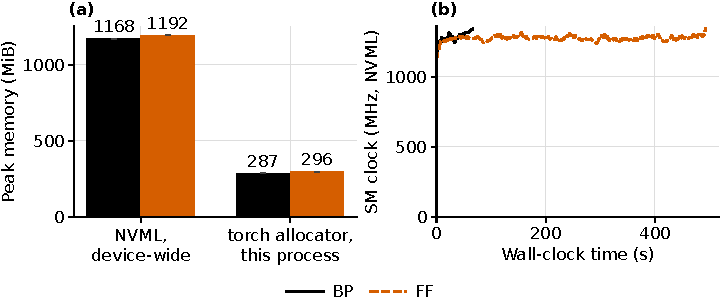
\includegraphics{plots/generated/fig_ff_resource.pdf}
  \vspace{-4pt}
  \caption{Hardware-level comparison of \FF{} against \BP{} on the
    Fashion-MNIST 4$\times$2000 MLP\@. (a) Peak memory read by two instruments:
    NVML reports the whole device including a CUDA context neither algorithm
    controls, while \texttt{torch.cuda.max\_memory\_allocated} reports this
    process. On both, \FF{} uses slightly \emph{more} memory than \BP{},
    refuting the presumed advantage of eliminating the backward pass.
    (b) SM clock (NVML, \SI{5}{\hertz}, rolling mean over \SI{10}{\second}) for
    the median-duration run of each method; both stay pinned near
    \SI{1300}{\mega\hertz}, so neither result is a throttling artefact.}
  \label{fig:ff_resource_utilization}
\end{figure}

\FloatBarrier

% ---- 5.2 ---------------------------------------------------
\needspace{3\baselineskip}
\subsection{\CaFo{}: A Structured Alternative with Acute Trade-offs}

The \CaFo{} algorithm, evaluated on its native 3-block CNN, revealed a
stark accuracy--efficiency trade-off contingent on its feature-learning
strategy. The \texttt{CaFo-Rand-CE} variant, using randomly
initialised fixed feature extractors, offered modest efficiency gains
but at the cost of a significant 13.23~percentage-point
accuracy drop on CIFAR-10 relative to \BP{}\@. The \texttt{CaFo-DFA-CE}
variant substantially improved accuracy but proved exceptionally
resource-intensive, consuming over four times more energy than
\BP{} on CIFAR-10. Table~\ref{tab:cafo_bp_cnn_summary} quantifies both
sides of this trade-off on that configuration.

% PROVISIONAL DATA: the three-seed figures below are recovered from the
% archived 2025 runs (NVIDIA driver 570.86.15) and were reconfirmed by
% reparsing the per-run logs. They must be regenerated on the current
% cluster (driver 595.71.05) before the paper is finalised.
\begin{table}[tb]
  \centering
  \caption{Performance and efficiency: \CaFo{} variants vs.\ \BP{} on the
    CIFAR-10 3-block CNN (mean~$\pm$~std, 3~runs).
    Better result in each column is shown in \textbf{bold}.
    Time and Energy cover full training to early stopping and include
    the \CaFoDFA{} block-pretraining stage.
    Memory is peak GPU allocation reported by NVML\@; it is a
    device-wide reading that includes the CUDA context and so separates
    the algorithms only weakly (see
    Section~\ref{sec:discussion_memory}).
    These figures are provisional: they were measured on an earlier
    revision of the cluster software stack and are pending regeneration
    in the environment reported above.}
  \label{tab:cafo_bp_cnn_summary}
  \setlength{\tabcolsep}{4pt}%
  \small
  \begin{tabular}{l
      S[table-format=2.2] @{\,$\pm$\,} S[table-format=1.2]
      S[table-format=4.2] @{\,$\pm$\,} S[table-format=2.2]
      S[table-format=2.2] @{\,$\pm$\,} S[table-format=1.2]
      S[table-format=4.0] @{\,$\pm$\,} S[table-format=1.0]}
    \toprule
    {Algorithm} &
      \multicolumn{2}{c}{Accuracy (\%)} &
      \multicolumn{2}{c}{Time (\si{\second})} &
      \multicolumn{2}{c}{Energy (\si{\watt\hour})} &
      \multicolumn{2}{c}{\shortstack[c]{Peak Mem \\ (\si{\mebibyte})}} \\
    \midrule
    \CaFoRand{}    & 66.09 & 0.32 & \bfseries 332.79 & \bfseries 61.94 & \bfseries 5.50 & \bfseries 1.00 & \bfseries 1014 & \bfseries 0 \\
    \CaFoDFA{}     & 77.60 & 0.25 & 1314.38 & 37.66 & 27.37 & 0.44 & 1128 & 0 \\
    \BP{} Baseline & \bfseries 79.32 & \bfseries 3.99 & 339.51 & 18.66 & 6.81 & 0.46 & 1114 & 0 \\
    \bottomrule
  \end{tabular}
\end{table}

Figure~\ref{fig:cafo_convergence} illustrates these distinct convergence
patterns on Fashion-MNIST. The flat initial segment in the
\CaFoDFA{} validation accuracy curve corresponds to the DFA
block-pretraining stage, during which the local predictors are not yet
active for the downstream task. This pretraining cost is included in
all reported \CaFoDFA{} time and energy figures, consistently
across all datasets.

\begin{figure}[tb]
  \centering
  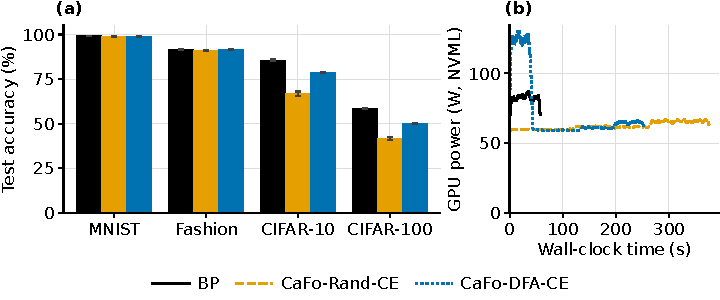
\includegraphics{plots/generated/fig_cafo_profile.pdf}
  \vspace{-4pt}
  \caption{\CaFo{} variants against \BP{}. (a) Final test accuracy across four
    datasets on the 3-block CNN, bootstrap 95\% CIs over $n=5$ seeds;
    \CaFoRand{} loses ground as the task hardens, exposing the limits of random
    fixed features. (b) GPU power (NVML, \SI{5}{\hertz}, rolling mean over
    \SI{5}{\second}) for the median-duration run on Fashion-MNIST. The upfront
    DFA block-pretraining stage is the elevated ${\approx}\SI{125}{\watt}$ regime
    over the first ${\approx}\SI{40}{\second}$; it is included in every reported
    energy and time figure. Per-epoch convergence curves are omitted because
    \CaFo{} trains each block's predictor independently and logs no global
    validation curve.}
  \label{fig:cafo_convergence}
\end{figure}

This highlights a critical design insight: while high-quality feature
representations are essential for accuracy, the DFA mechanism used by
\CaFoDFA{} to learn them is computationally prohibitive.
The supplementary material provides full comparative results
across all datasets.

% ---- 5.3 ---------------------------------------------------
\needspace{3\baselineskip}
\subsection{\MF{}: A Superior Accuracy--Efficiency Profile on MLP
Architectures}

The Mono-Forward algorithm consistently matched or surpassed \BP{}
classification accuracy on all tested MLP architectures
(Table~\ref{tab:mf_bp_perf_eff_summary}). The accuracy advantage was
+0.51~pp on Fashion-MNIST and +1.21~pp on
CIFAR-10, the most complex tested configuration.
Note that CIFAR-10 accuracy for MLP architectures is substantially lower
than CNN-based state-of-the-art owing to the elimination of spatial
structure via flattening; the comparison here is strictly between an
MLP-based \MF{} and an MLP-based \BP{} baseline on identical architectures.
The accuracy margins are modest, and as noted in the statistical note
above, with only three runs their statistical robustness cannot be
formally established; they are empirical observations, not confirmed
claims.

\begin{table}[tb]
  \centering
  \caption{Performance and efficiency: \MF{} vs.\ \BP{} on the CIFAR-10
    3$\times$2000 MLP (mean~$\pm$~std, 3~runs; seeds 42, 123, 7).
    Better result in each column is shown in \textbf{bold}.
    Time and Energy cover full training to early stopping.
    Memory is peak GPU allocation reported by NVML\@.
    CIFAR-10 inputs are flattened to 3072-dimensional vectors
    following the \MF{} protocol. Peak Mem bold reflects a $\sim$5\%
    margin; see Section~\ref{sec:discussion_memory} for discussion.}
  \label{tab:mf_bp_perf_eff_summary}
  \setlength{\tabcolsep}{4pt}%
  \small
  \begin{tabular}{l
      S[table-format=2.2] @{\,$\pm$\,} S[table-format=1.2]
      S[table-format=3.2] @{\,$\pm$\,} S[table-format=1.1]
      S[table-format=1.2] @{\,$\pm$\,} S[table-format=1.2]
      S[table-format=4.0] @{\,$\pm$\,} S[table-format=1.0]}
    \toprule
    {Algorithm} &
      \multicolumn{2}{c}{Accuracy (\%)} &
      \multicolumn{2}{c}{Time (\si{\second})} &
      \multicolumn{2}{c}{Energy (\si{\watt\hour})} &
      \multicolumn{2}{c}{\shortstack[c]{Peak Mem \\ (\si{\mebibyte})}} \\
    \midrule
    \MF{}          & \bfseries 62.34 & \bfseries 0.28 & \bfseries 177.70 & \bfseries 7.1 & \bfseries 3.17 & \bfseries 0.12 & \bfseries 1120 & \bfseries 9 \\
    \BP{} Baseline & 61.13 & 0.35 & 268.45 & 8.1 & 5.35 & 0.19 & 1184 & 5 \\
    \bottomrule
  \end{tabular}
\end{table}

{\looseness=-1
On Fashion-MNIST, \MF{} achieved higher accuracy (+0.51~pp) at the cost of
modestly increased training time (+18.20\%) and energy consumption
(+9.90\% relative to \BP{}), as reported in
the supplementary material. This configuration represents
an empirical trade-off: higher accuracy is accompanied by slightly
higher resource use. On CIFAR-10, the most demanding tested
configuration, \MF{} was 33.81\% faster and consumed
40.78\% less energy than \BP{} while achieving higher accuracy,
representing the strongest case for \MF{}'s efficiency advantage.
\par}

{\looseness=-1
Hardware monitoring on the CIFAR-10 task shows what \MF{}'s local training
regime actually does to the device
(Figure~\ref{fig:mf_hardware_and_memory}). \MF{} draws less power and keeps
the GPU roughly half as busy as \BP{}, but it stays on the device almost four
times as long, so the lower instantaneous draw does not translate into lower
energy. Its per-layer stages are visible as steps in both the utilisation and
the memory trace. The device-wide memory reading separates the two algorithms
by little because it includes the fixed CUDA context that neither of them
controls; Figure~\ref{fig:time_memory_frontier} reports the per-process figure
instead.
\par}

\begin{figure}[tb]
  \centering
  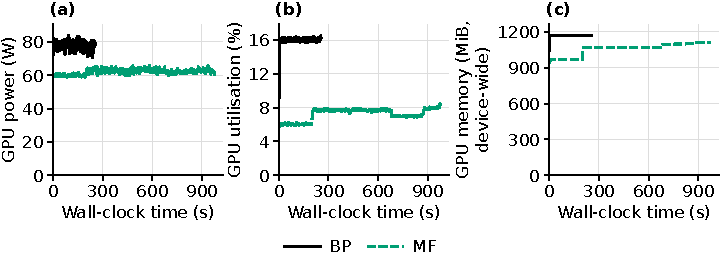
\includegraphics{plots/generated/fig_mf_hardware.pdf}
  \vspace{-4pt}
  \caption{Hardware monitoring of the \BP{}$\to$\MF{} ladder on the CIFAR-10
    3$\times$2000 MLP, median-duration run per rung. All three traces are NVML
    at \SI{5}{\hertz} (rolling mean over \SI{5}{\second}); none is a
    Weights~\&~Biases system panel. (a) \MF{} draws roughly
    \SI{61}{\watt} against \BP{}'s \SI{78}{\watt}, but for almost four times as
    long, so the area under the curve---the energy---is far larger.
    (b)~Utilisation and (c)~device memory expose \MF{}'s per-layer stages as
    visible steps. The device-memory reading includes the fixed CUDA context,
    which is why the rungs separate by so little; see
    Figure~\ref{fig:time_memory_frontier} for the per-process figure.}
  \label{fig:mf_hardware_and_memory}
\end{figure}

\needspace{3\baselineskip}
Figure~\ref{fig:mf_bp_cifar10_mlp_conv_curves} shows where that cost is
actually spent. Every rung of the ladder draws close to the same power, so
energy tracks wall-clock time almost exactly and the ranking of the rungs by
energy is the ranking by duration. \MF{} nonetheless reaches higher accuracy
than \BP{} on identical architectures; we discuss a possible regularisation
hypothesis in Section~\ref{sec:discussion_why_mf}.

\begin{figure}[tb]
  \centering
  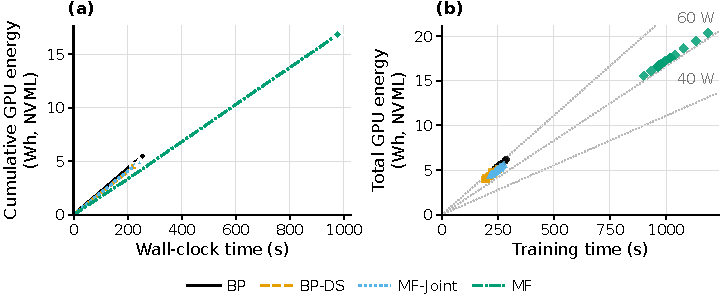
\includegraphics{plots/generated/fig_mf_bp_cost_curves.pdf}
  \vspace{-4pt}
  \caption{What a training run costs, on the CIFAR-10 3$\times$2000 MLP\@.
    (a) Cumulative GPU energy against wall-clock time for the
    median-duration run of each ladder rung, integrated from the NVML power
    trace; the end marker is the total. (b) Every seed, total energy against
    training time, with iso-power guides. All four rungs sit near the same
    power draw, so energy is set almost entirely by how long the run takes.
    A validation-loss comparison is not shown: \MF{} optimises a separate local
    objective per layer and logs no global validation curve, so no such series
    exists for it in the run archive.}
  \label{fig:mf_bp_cifar10_mlp_conv_curves}
\end{figure}

{\looseness=-1
A complete summary comparing the relative performance and efficiency of
each algorithm against its fair \BP{} baseline across all tested
configurations is presented in the supplementary material.
\par}

% ---- 5.4 ---------------------------------------------------
\needspace{3\baselineskip}
\subsection{Where the Cost Comes From}
\label{sec:ladder}

Attributing \MF{}'s cost to \MF{} as a whole explains nothing. We therefore
interpolate between \BP{} and \MF{} in single-change steps---auxiliary
supervision, the learned readout $M_L$, gradient locality, and, where
activations can be cached, two caching strategies---and measure each step
separately (Figure~\ref{fig:ladder_waterfall}). One step dominates. Detaching
the gradient at every layer boundary adds between \num{228} and \num{272}~pp of
\BP{}'s energy across the four configurations, while auxiliary supervision and
the readout together move it by at most \num{40}~pp and on the two CIFAR tasks
partly cancel. The overhead is not an implementation detail that tuning will
remove: it is the price of locality itself.

Caching activations is the obvious remedy, and it does not work
(Figure~\ref{fig:time_memory_frontier}). Caching on the device buys no time and
costs several times the per-process memory; caching on the host adds
\num{261}~pp of \BP{}'s energy on MNIST and \num{441}~pp on Fashion-MNIST on
top of \MF{}'s own overhead. Neither strategy reaches a point that \MF{}
without caching does not already dominate.

Finally, we report accuracy differences as intervals rather than as verdicts
(Figure~\ref{fig:equivalence_forest}). Of \num{28} contrasts, eleven are
equivalent within the preregistered margin, sixteen are different, and one is
inconclusive: \CaFoDFA{} against \BP{} on the Fashion-MNIST CNN, whose interval
spans $[\num{-0.03},\num{+0.61}]$~pp at five seeds---wide enough to contain
both the margin and values well outside it. We mark such a contrast
inconclusive rather than reading it as evidence of parity.

\begin{figure}[tb]
  \centering
  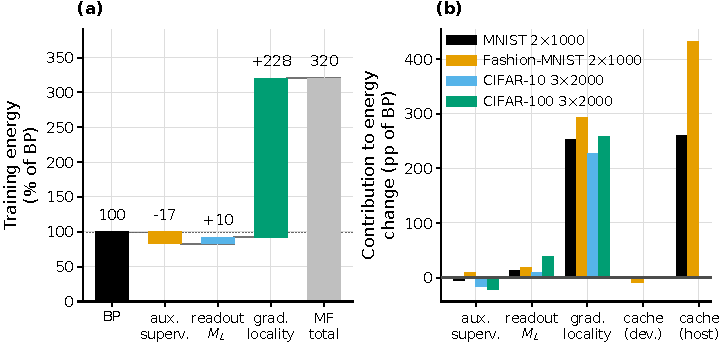
\includegraphics{plots/generated/fig_ladder_waterfall.pdf}
  \vspace{-4pt}
  \caption{Decomposition of the \BP{}$\to$\MF{} energy change into five
    single-change steps. (a) Cumulative GPU energy on the CIFAR-10
    3$\times$2000 MLP as a percentage of \BP{}, each bar one rung transition.
    (b) The same per-step contributions for all four configurations. Gradient
    locality accounts for essentially the whole increase everywhere. Energy is
    the trapezoidal integral of the NVML power trace (\SI{5}{\hertz}); bars are
    seed means over \numrange{20}{122} seeds per rung.}
  \label{fig:ladder_waterfall}
\end{figure}

\begin{figure}[tb]
  \centering
  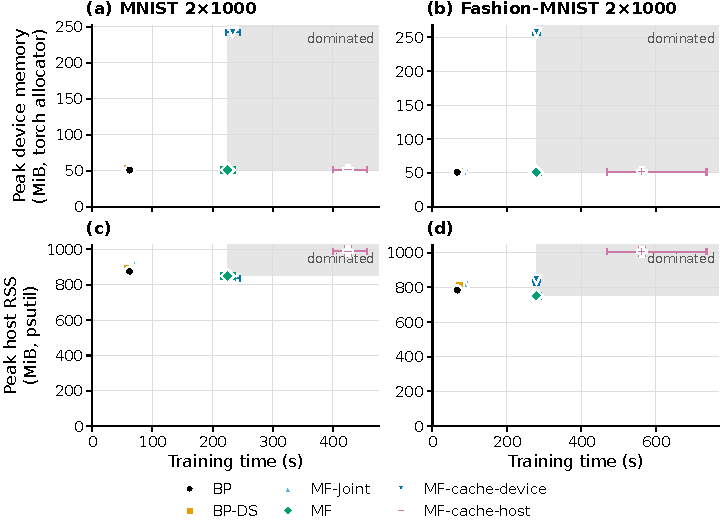
\includegraphics{plots/generated/fig_time_memory_frontier.pdf}
  \vspace{-4pt}
  \caption{Time against memory for \BP{} and the three \MF{} caching
    strategies. Top row: peak memory allocated by this process
    (\texttt{torch.cuda.max\_memory\_allocated}), which excludes the fixed CUDA
    context. Bottom row: peak host resident set size (psutil). The shaded
    quadrant is the region dominated by \MF{} without caching---worse on both
    axes. Both caching strategies fall inside it, so neither is on the frontier.
    Markers are seed means with bootstrap 95\% CIs, \numrange{20}{122} seeds
    per point.}
  \label{fig:time_memory_frontier}
\end{figure}

\begin{figure}[tb]
  \centering
  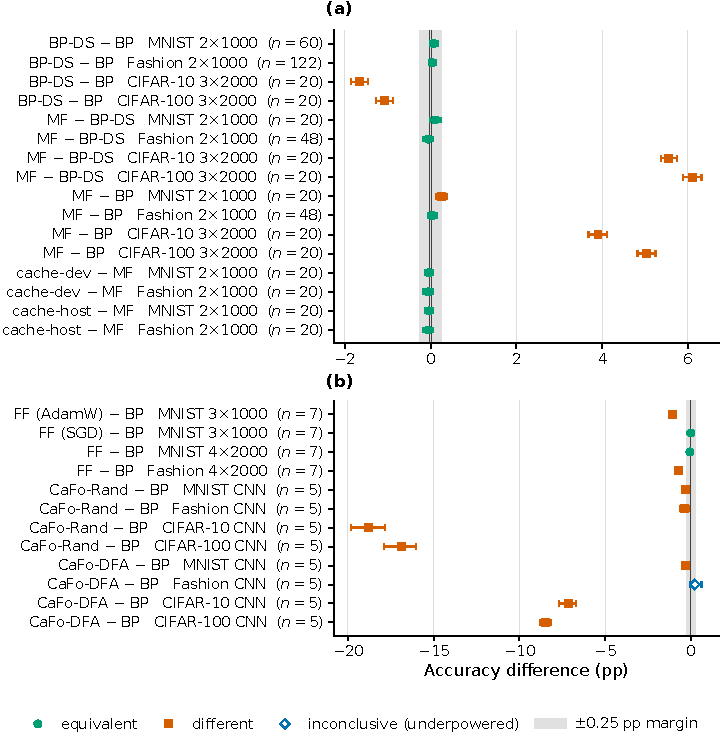
\includegraphics{plots/generated/fig_equivalence_forest.pdf}
  \vspace{-4pt}
  \caption{Paired differences in final test accuracy, bootstrap 95\% CIs
    (\num{10000} resamples, fixed seed). The shaded band is the preregistered
    $\pm$\num{0.25}~pp equivalence margin. A contrast is resolved as equivalent
    only when its whole interval lies inside the band, and as different only
    when the interval excludes zero; everything else is marked inconclusive.
    Paired seed counts are given per row. (a) The \BP{}$\to$\MF{}
    ladder. (b) \FF{} and \CaFo{} against their matched \BP{} baselines.}
  \label{fig:equivalence_forest}
\end{figure}

\FloatBarrier

% ============================================================
\section{Discussion}
\label{sec:discussion}
% ============================================================

We interpret the empirical results, discuss methodological limitations,
and draw implications for future work. Where interpretations go beyond
the data, we label them explicitly as hypotheses.

% ---- 6.1 ---------------------------------------------------
\needspace{3\baselineskip}
\subsection{Why \MF{} Succeeds: A Regularisation Hypothesis}
\label{sec:discussion_why_mf}

{\looseness=-1
\FF{}'s inefficiency traces to its indirect goodness signal and contrastive
data generation, resulting in slow convergence and poor GPU utilisation
(Section~\ref{sec:experiments}). \CaFo{}'s DFA block-pretraining resolves
the feature quality problem but at unacceptable energy cost, suggesting
that a direct supervisory signal is necessary but that DFA is not the
right mechanism. \MF{}'s local projection matrices provide exactly such a
direct signal — a local cross-entropy loss at each layer — with minimal
overhead. The mechanism is closely related to the local auxiliary losses
studied by \cite{ren2023scaling} and \cite{ishikawa2025local}. Of particular
relevance, \cite{ishikawa2025local} analyse local loss optimisation in the infinite-width limit and show
that greedy layer-wise training can reduce the effective complexity of the learned
representation in ways that support generalisation.
\par}

{\looseness=-1
This theoretical result motivates the \emph{regularisation hypothesis}
for \MF{}'s accuracy advantage: that the layer-wise, greedy nature of
\MF{}'s optimisation implicitly constrains the representational complexity
of each layer, guiding the model toward a solution with better
generalisation properties than \BP{}'s global, joint optimisation. The
lower final validation loss observed for \MF{} in
Figure~\ref{fig:mf_bp_cifar10_mlp_conv_curves} is consistent with this
hypothesis. We emphasise that this remains a hypothesis: confirming it
would require diagnostic experiments such as measuring the
train--validation accuracy gap across training, computing sharpness
metrics (e.g., $\lambda_{\max}$ of the loss Hessian), or comparing
generalisation bounds under the two optimisation regimes. We leave such
analysis to future work.
\par}

% ---- 6.2 ---------------------------------------------------
\needspace{3\baselineskip}
\subsection{Rethinking Memory Efficiency in BP-Free Learning}
\label{sec:discussion_memory}

A critical finding is that eliminating the backward pass does not
automatically guarantee superior memory efficiency. While
\CaFoRand{} showed modest memory savings (approximately 6--9\%
across datasets), both \FF{} and \CaFoDFA{} consumed \emph{more}
memory than their \BP{} baselines. Even \MF{}'s memory advantage on larger
MLPs was modest at approximately 5\%.

This occurs because the practical overhead of algorithm-specific
components, specifically \FF{}'s dual data streams, \MF{}'s per-layer projection
matrices, and \CaFoDFA{}'s DFA feedback tensors, can counteract the
theoretical savings from not storing activations for the backward pass.
Peak memory as reported by NVML captures GPU-resident tensor
allocations; note that PyTorch's memory allocator may retain freed
blocks in a pool, so peak allocation can differ from the maximum
simultaneously-live tensor memory. These findings underscore the
necessity of direct hardware measurement rather than theoretical
analysis alone.

% ---- 6.3 ---------------------------------------------------
\needspace{3\baselineskip}
\subsection{Implications for Efficient Training and Hardware Co-Design}
\label{sec:discussion_hardware_codesign}

{\looseness=-1
\MF{}'s energy reduction on CIFAR-10 (approximately 41\%) and training
time reduction (approximately 34\%) relative to a fairly tuned \BP{}
baseline are meaningful results for the specific setting studied: MLP
architectures on standard vision benchmarks on an
NVIDIA A100-SXM4-40GB GPU\@. Whether these advantages persist on
larger networks, different hardware platforms (consumer GPUs, TPUs,
edge devices), or other data domains is unknown and represents an
important open question.
\par}

{\looseness=-1
If forward-only algorithms like \MF{} prove effective at larger scales,
they could motivate hardware designs with simpler memory subsystems
without activation checkpointing and compute pipelines optimised for
sequential, layer-local operations, a speculative but well-motivated
direction. Extrapolating the present savings to a broader sustainability
claim would require demonstrating similar advantages at the scale where
energy costs are societally
significant~\cite{strubell2019energy,patterson2021carbon}.
\par}

% ---- 6.4 ---------------------------------------------------
\needspace{5\baselineskip}
\subsection{Limitations}
\label{sec:limitations}

We provide an explicit, comprehensive account of this study's
limitations:
\begin{enumerate}
  \item \textbf{Architecture and scale.} Results apply to 2--4-layer MLP
        architectures (\FF{} and \MF{}) and a 3-block CNN (\CaFo{});
        performance on deeper CNNs, residual networks, transformers, or
        attention-based architectures is entirely untested. Networks are
        moderately sized (up to 4 layers of 2000 units); the behaviour
        of \MF{} and \FF{} under increasing depth, width, or dataset
        complexity is unknown, though prior work on local-loss
        methods~\cite{ren2023scaling} suggests scalability.
  \item \textbf{Datasets.} MNIST, Fashion-MNIST, CIFAR-10, and
        CIFAR-100 are well-established but small-scale benchmarks.
        CIFAR-10 and CIFAR-100 inputs are flattened to 1-D vectors for
        MLP experiments, which eliminates spatial structure. Findings
        may not reflect behaviour on larger or more complex datasets.
  \item \textbf{Hardware specificity.} All hardware results are specific
        to the NVIDIA A100-SXM4-40GB on the Athena cluster. Results may
        differ significantly on consumer GPUs (e.g., RTX~4090), TPUs,
        or edge hardware.
  \item \textbf{Statistical robustness.} Three runs are insufficient to
        establish statistical significance at conventional thresholds,
        especially for small accuracy margins (e.g., +0.09~pp on MNIST);
        the \MF{} MNIST advantage in particular should be interpreted with
        considerable caution.
  \item \textbf{Hyperparameter search confound.} Each algorithm
        underwent independent Optuna tuning. Differences in performance
        may partly reflect better hyperparameter discovery rather than
        intrinsic algorithmic superiority. The hyperparameter search
        cost itself was not included in the reported training time and
        energy figures; for slow algorithms like \FF{}, the 50-trial Optuna
        search overhead is substantial and should be considered in any
        total-cost assessment.
  \item \textbf{Missing deep-supervision baseline.} \MF{} introduces
        per-layer projection matrices and local cross-entropy losses,
        which both enable the BP-free training signal \emph{and} add
        additional parameter capacity and supervision depth relative to
        the standard \BP{} baseline. A \BP{} network with equivalent
        per-layer auxiliary heads (\texttt{BP-DS};
        ``deep supervision''~\cite{lee2015deeply}) — adding projection
        heads of identical dimension with auxiliary cross-entropy losses
        at each layer and training end-to-end — would allow attribution
        of \MF{}'s accuracy advantage specifically to the forward-only
        training regime. We were unable to complete this comparison
        within the present submission and include it as a priority item
        for future work. All efficiency comparisons (energy, time,
        memory) remain interpretable regardless.
  \item \textbf{Inconsistent Fashion-MNIST \MF{} result.} On
        Fashion-MNIST, \MF{} incurred a 9.90\% increase in energy relative
        to \BP{}\@. This is inconsistent with the efficiency gains observed
        on CIFAR-10 and CIFAR-100. The cause is not fully understood; it
        may reflect dataset-specific convergence behaviour or
        hyperparameter interactions on the smaller network
        (2$\times$1000 MLP). This result qualifies any claim of
        consistent efficiency superiority across all configurations.
  \item \textbf{Scope of contribution.} This paper's primary
        contribution is evaluative, not algorithmic; the benchmarking
        framework, fair comparison conditions, and hardware-level
        measurements are our contribution. The algorithms (\FF{}, \CaFo{},
        \MF{}) are previously
        published~\cite{hinton2022forward,zhao2023cafo,gong2025mono}.
\end{enumerate}

\FloatBarrier

% ============================================================
\needspace{4\baselineskip}
\section{Conclusion}
\label{sec:conclusion}
% ============================================================

We presented a rigorous, hardware-validated benchmarking study of three
forward-only, BP-free training algorithms, namely \FF{}, \CaFo{}, and
\MF{}, evaluated against fairly tuned \BP{} baselines under a principled
fairness framework on MLP and CNN architectures across four standard
vision benchmarks.

{\looseness=1
On its native MLP architectures, \MF{} consistently matched or surpassed
\BP{} in classification accuracy across all tested configurations,
achieving up to 41\% lower energy consumption and up to 34\% faster
training on CIFAR-10. These findings challenge the assumption that
global end-to-end optimisation is necessary for competitive accuracy on
these architectures and establish \MF{} as a practically viable training
algorithm for this setting. By contrast, \FF{} incurred prohibitive
efficiency costs despite moderate accuracy gains, and \CaFo{} faced an
acute accuracy--efficiency trade-off that limited its practical utility
without the expensive DFA pretraining stage.
\par}

{\looseness=-1
Importantly, these results are specific to MLP architectures on
standard, small-scale benchmarks on a single GPU platform. The finding
that BP-free training can match or exceed \BP{}'s accuracy and efficiency
cannot be extrapolated to larger models, other architectures, or other
hardware without further investigation. The absence of a
deep-supervision \BP{} baseline (\texttt{BP-DS}) is a notable gap that
future work should address to isolate the algorithmic contribution of
forward-only training.
\par}

{\looseness=-1
Within its established scope, this work provides a reproducible
benchmarking framework, hardware-level efficiency profiles, and an
empirical re-evaluation of memory efficiency that together offer a more
rigorous empirical foundation for evaluating BP-free methods than was
previously available.
\par}

\subsubsection{\ackname}
This work was supported by the Ministry of Science and Higher Education of
Poland and by the National Science Centre (NCN), Poland, under grant OPUS-29,
DEC-2025/57/B/ST6/04377. The authors wish to thank the PLGrid Infrastructure
and ACK Cyfronet AGH for providing the computational resources on the Athena
cluster, which were indispensable for this work. The research was conducted as
part of a~master's thesis by \mbox{Przemys{\l}aw} Spyra, under the supervision
of Witold Dzwinel. \mbox{Przemys{\l}aw} Spyra was responsible for the
development and implementation of the methodology, experiments, and analysis.
Witold Dzwinel provided conceptual guidance, critical feedback, and helped shape
the direction and presentation of the work. We gratefully acknowledge the AGH
University of Krakow for providing the institutional support and academic
environment that made this research possible.

\subsection{Code Repository}
% FIX #5: Renamed label from \label{app:repository} to \label{sec:repository}.
% The subsection now lives in the main paper body, not in an appendix;
% the "app:" prefix was semantically misleading. No \ref{} calls in
% main.tex pointed to this label, so no further updates are required here.
\label{sec:repository}

To ensure full reproducibility, we provide the complete research
artifacts associated with this work. This includes the full source code,
all configuration files, selected hyperparameter YAML specifications,
and per-run experimental logs. In addition, all appendix material
previously included in the manuscript has been moved to the repository
as an online appendix.

\begin{center}
  \url{https://github.com/Przemyslaw11/BeyondBackpropagation}
\end{center}

% ============================================================
%  Bibliography
% ============================================================
\bibliographystyle{splncs04}
\begin{sloppypar}
\bibliography{bibliography}
\end{sloppypar}

\end{document}
